\section{Verificaciones}

En esta sección se va a justificar mediante las simulaciones necesarias que el funcionamiento del circuito es el correcto.
Primero, se comprueba que la tensión de salida sin carga es igual a la esperada. En la figura \ref{Vout_50Hz} se puede ver que, al transcurrir
un tiempo de aproximadamente 5 segundos, la tensión de salida se estabiliza en $3101V$, valor que supone un error mínimo del $0,33\%$
respecto a la tensión de salida esperada sin carga ($3111,27V$), como se puede ver en la siguiente expresión:

\begin{equation}
    E_{V_{noload}} = \frac{3111,27V - 3101V}{3111,27V} \cdot 100 = 0,33\%
\end{equation}

\begin{figure}[H]
    \centering
    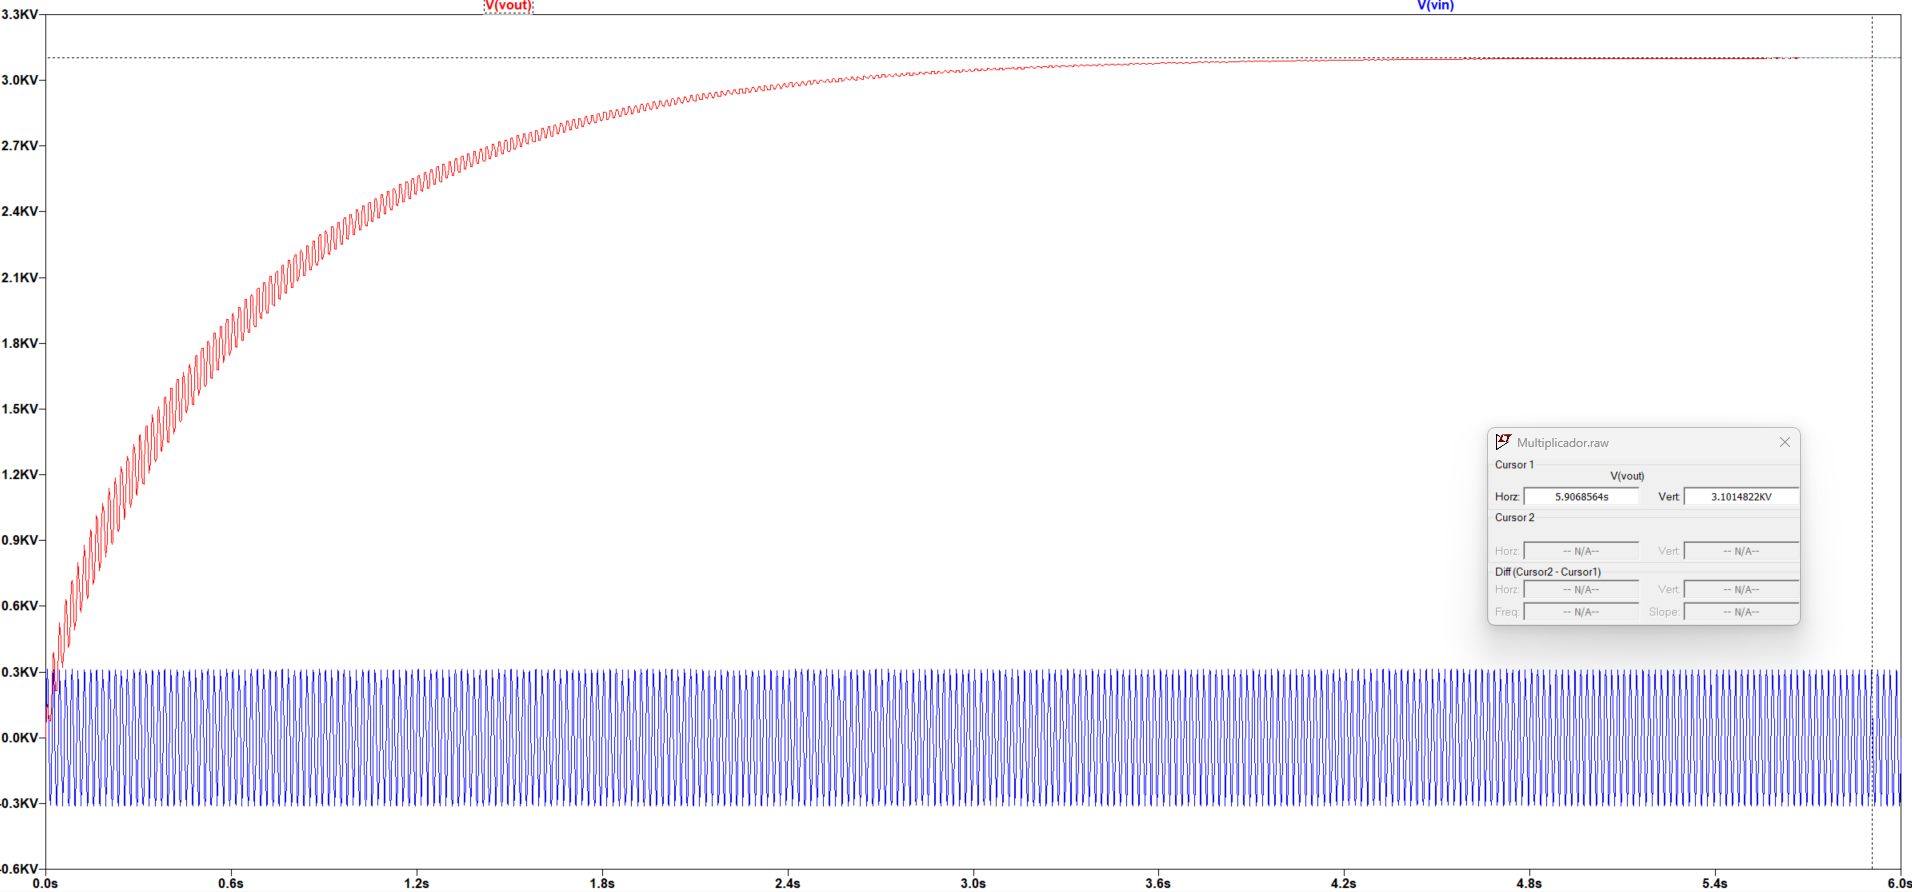
\includegraphics[width=1\textwidth]{Imagenes_alvaro/Vout_50hz.png}
    \caption{Tensión de salida y entrada a 50Hz (sin carga)}
    \label{Vout_50hz}
\end{figure}

Además, podemos garantizar que la tensión obtenida está dentro del rango de tensión de salida especificado, puesto que la tensión máxima 
establecida ($5\%$ de $3kV$) es de $3150V$.

Tras comprobar que el circuito funciona correctamente, pasamos a conectar la carga y el circuito de medida.
Respecto del caso anterior, el tiempo de establecimiento es similar y no relevante puesto que no existe ningún requerimiento respecto del mismo, por lo que
se pasa a analizar la tensión de salida en estacionario, obteniendo el resultado \ref{Vout_50hz_load}.

\begin{figure}[H]
    \centering
    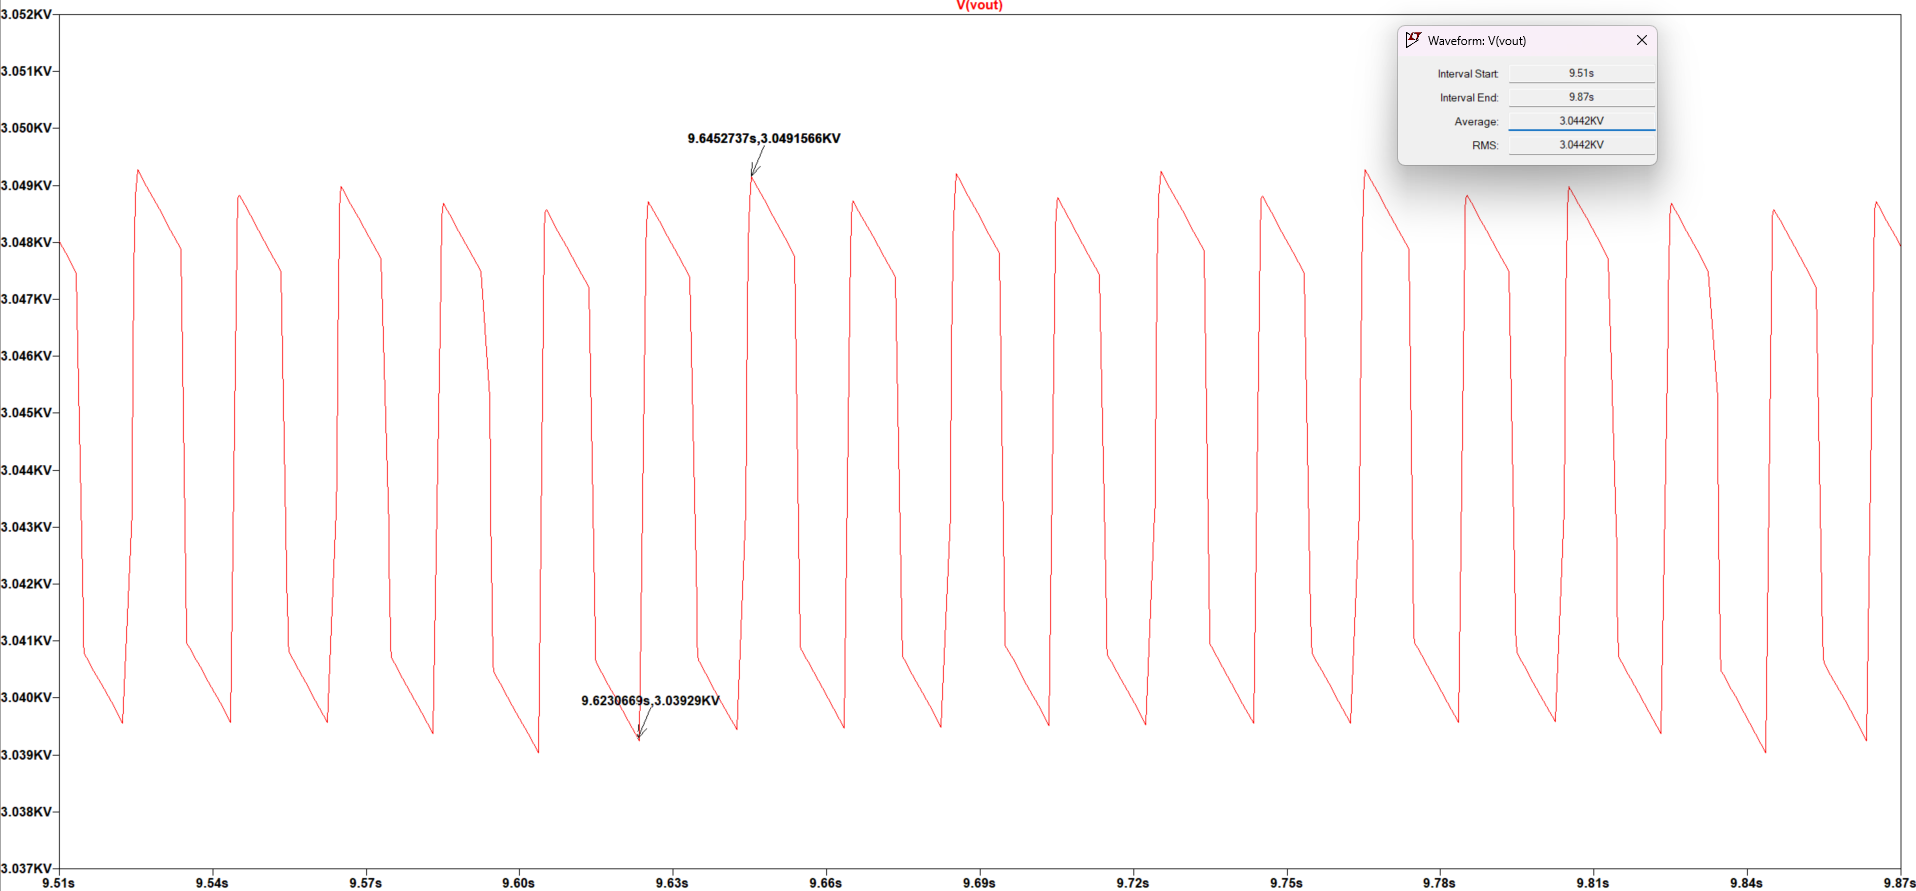
\includegraphics[width=1\textwidth]{Imagenes_alvaro/Vout_50hz_load.png}
    \caption{Tensión de salida y entrada a 50Hz con carga}
    \label{Vout_50hz_load}
\end{figure}

Como se puede ver en la figura \ref{Vout_50hz_load}, se obtiene una tensión media de $3044V$, una tensión máxima de $3049V$ y una tensión
mínima de $3039V$. De esta manera, se puede garantizar que el requisito de rizado de $10V$ para 50Hz sí se cumple, y el error obtenido 
para la tensión media es mínimo:

\begin{equation}
    E_{V_{load}} = \frac{3047,93V - 3044V}{3047,93V} \cdot 100 = 0,13\%
\end{equation}